\documentclass{sig-alternate}
%\usepackage{latex8}
\usepackage{times}
%\usepackage{algorithm}
%\usepackage{algorithmic}
\usepackage{graphicx}
\usepackage{epsfig}
\usepackage{color}
\usepackage{amssymb}
\usepackage{flushend}
\usepackage{cite,float}

\newtheorem{theorem}{Theorem}[section]
\newtheorem{lemma}[theorem]{Lemma}
\newtheorem{proposition}[theorem]{Proposition}
\newtheorem{corollary}[theorem]{Corollary}

\newenvironment{definition}[1][Definition]{\begin{trivlist}
\item[\hskip \labelsep {\bfseries #1}]}{\end{trivlist}}
\newenvironment{example}[1][Example]{\begin{trivlist}
\item[\hskip \labelsep {\bfseries #1}]}{\end{trivlist}}
\newenvironment{remark}[1][Remark]{\begin{trivlist}
\item[\hskip \labelsep {\bfseries #1}]}{\end{trivlist}}

\begin{document}

\title{Agile Information Acquisition and Management System for Magnetized Dusty Plasma Experiment Project}


\numberofauthors{3}

\author{
\alignauthor Chih-Jye Wang\\
      \affaddr{Dept. of Computer Science and Software Engineering}\\
      \affaddr{Auburn University}\\
     \affaddr{Auburn, AL 36849, USA}\\
      \email{wangchj@auburn.edu}
\alignauthor Edward Thomas, Jr\\
      \affaddr{Dept. of Physics}\\
      \affaddr{Auburn University}\\
     \affaddr{Auburn, AL 36849, USA}\\
      \email{thomaed@auburn.edu}
\alignauthor Darrick Artis\\
      \affaddr{Dept. of Physics}\\
      \affaddr{Auburn University}\\
     \affaddr{Auburn, AL 36849, USA}\\
      \email{doa0003@auburn.edu}
%\alignauthor Wei-Shinn Ku\\
%       \affaddr{Dept. of Computer Science and Software Engineering}\\
%       \affaddr{Auburn University}\\
%      \affaddr{Auburn, AL 36849, USA}\\
%       \email{weishinn@auburn.edu}
}


%\conferenceinfo{ACM GIS'09,} {November 4-6, 2009. Seattle, WA, USA}
%\CopyrightYear{2010} \crdata{ISBN 978-1-60558-649-6/09/11}


\maketitle

\begin{abstract}
An agile information acquisition and management system for the Magnetized Dusty Experiment is presented. The data storage of the system is divided into two categories. The first is the research data which include time-series pulse data and video data from the experiment. This bulk research data is stored as normal files on a file system. The second category is the research metadata, which precisely describes the setup information as well as instrumental set-points of an experiment. We use a relational database to store this data. Using a relational database allows us to impose relationships across different runs of experiments at the same time allow us to store mixture of flat and hierarchical data. In addition the database allows the research to specify precise queries to find the data of interest. This report describes the structure of the research data as well as the metadata database. In addition, a web interface to the database is also presented.
\end{abstract}

\category{H.2.8}{Database Management}{Database Application}[spatial databases and GIS]
\terms{Algorithms and Experimentation}
\keywords{Location-based services, location privacy and spatial cloaking} % NOT required for Proceedings

\section{Introduction}
This report describes information management system for the Magnetized Dusty Plasma Experiment (MDPX)\cite{0741-3335-54-12-124034,6414662} project at Auburn University. The primary purpose of the system is to store and retrieve experiment calibration, setup, and summarized research data. The following are the design motivation of the database system:

\begin{itemize}
\item Fast retrieval of stored data that has not been a goal of older database systems .
\item Sophisticated data search and filtering capability, which allows researchers to form relations and hypothetical research proposals across multiple experimental setups and scenarios.
\end{itemize}

In addition, the system was designed to be agile and modular. New features can be easily added to the database, and database can be accessed through any software package or language that supports data access via SQL\footnote{http://en.wikipedia.org/wiki/SQL}.

The system is roughly divided into 3 major parts as shown in Figure~\ref{fig:overview}: relational database management system, LabVIEW\footnote{http://www.ni.com/labview/} control and data acquisition subsystem, and web-based data manager. Our LabVIEW control software interfaces with (for the lack of proper technical term) the dusty plasma experimental hardware and stores setup and experiment data into the database. The web interface allows researchers and operators to monitor and search acquired data from experiment runs. This report will cover the design of the database and overview the capability of the web interface. The LabVIEW control 

\begin{figure}[h!]
\begin{center}
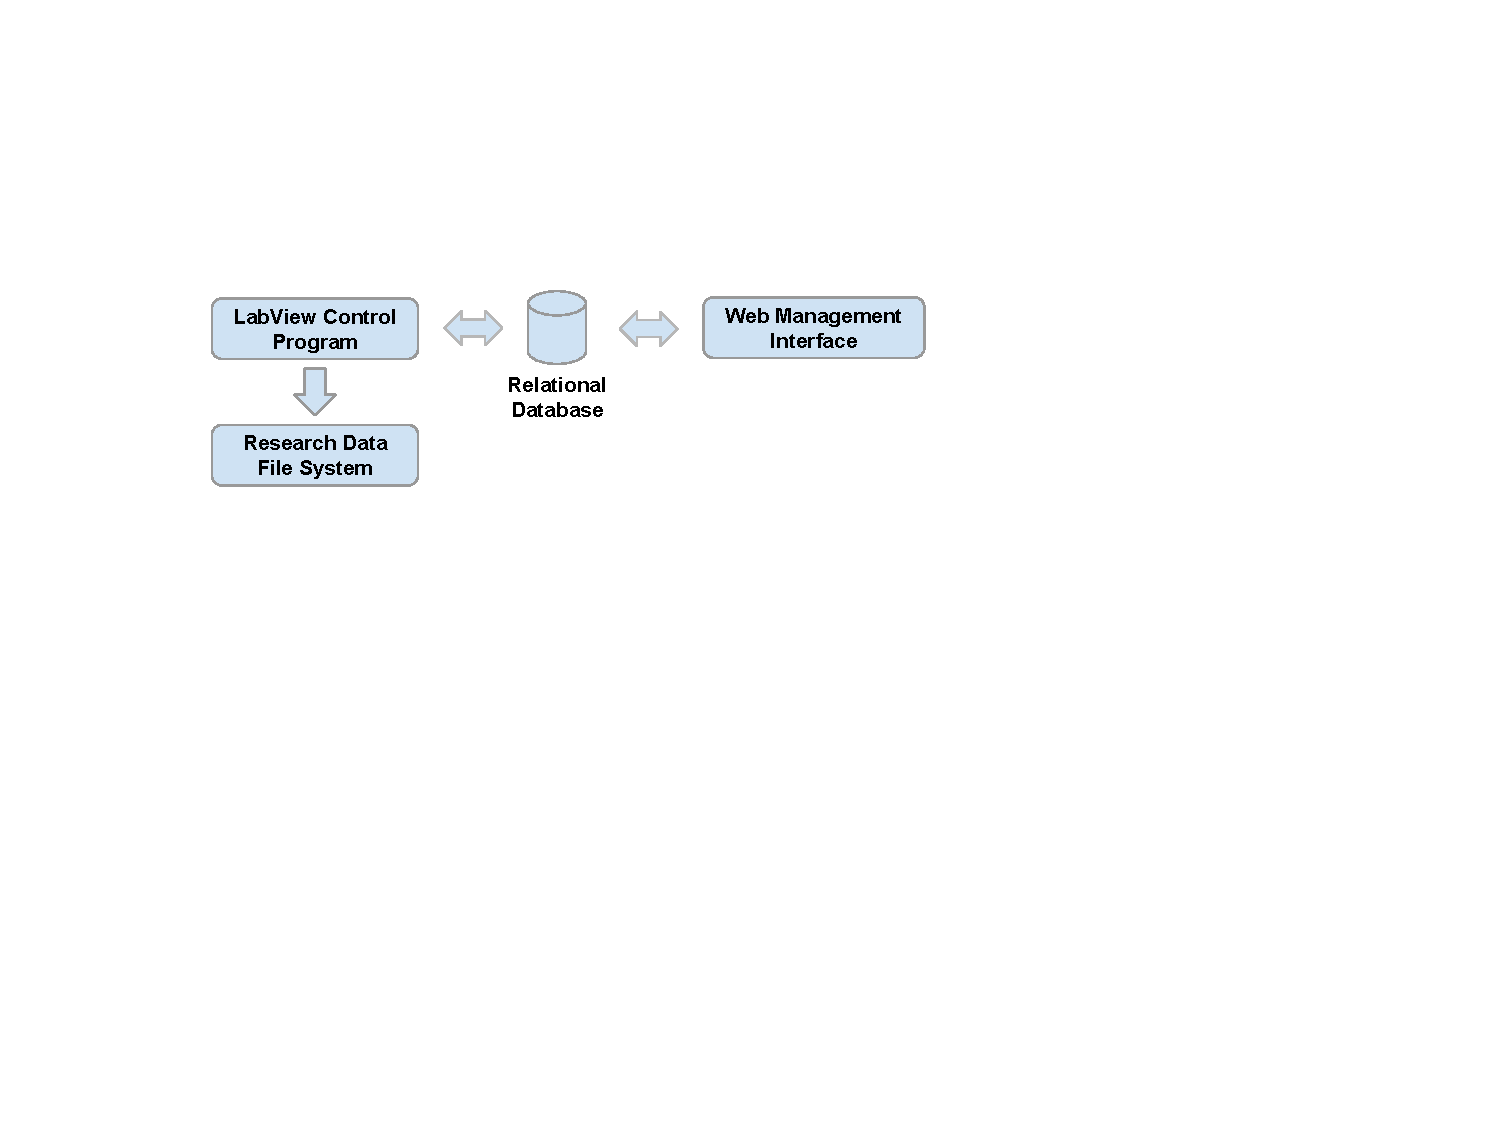
\includegraphics[width=3.2in]{overview.pdf}
\caption{Data acquisition system overview.\label{fig:overview}}
\end{center}
\end{figure}

[Report outline]


\section{Comparative Database Systems}


\section{Data Storage}

The acquired experiment research data is split into two categories: experiment metadata and bulk research data. Experiment metadata precisely describe repeatable experimental parameters. This information contains:

\begin{itemize}
\item Calibration (?)
\item Parts
\item Part setup
\item Parametric set-points
\item If experiment is a systematic scan from a control program
\item Recorded summarized research data
\item Storage location of bulk research data
\item User management
\end{itemize}

The metadata is stored in a MySQL\footnote{http://www.mysql.com/} relational database. There are three main reasons that we use MySQL to store this data. The first is that MySQL allows us to impose relationships among experiments. A simple relationship would be two experiments sharing the same part setup (but not necessary the same set-points). Second, MySQL supports broad range of data searching capabilities, which facilitates researchers to quickly find experiments of interest. The final reason is that MySQL has great performance of data searching.  MySQL is the most used relational database management system with proven data storage and retrieval performance. In addition, according to a publication by Princeton Plasma Physics Laboratory on data management for Plasma Physics Databases\cite{Davis2004183}, a relational database is several factors faster than MDSplus\cite{4994733} database with reasonable data compression ratio. The metadata can be thought as a research data index to find proper experiments.

The second broad category of data is the bulk research data. These include dense time-series pulse measurements, and video files. Much of these files are large files and they are stored on file system outside of the relational database. The location for each experiment is easily searchable via metadata database.


\subsection{Metadata Database}

The database is a relational database that is used to store and to perform complex analytical query operations of the metadata. Figure~\ref{fig:schema} in Appendix~\ref{app_db_schema} shows the database schema that contains all the tables.

\emph{Note}: In addition to the tables shown in Figure 2, the database also contains a set of user defined views that are currently used by the web interface to show data merged from different tables.

The database tables are divided into 4 groups that are described in this section. 


\subsubsection{Catalog}

The \emph{catalog} consists of a set of tables that keeps an inventory of parts and materials that we have at our facility and are used in the experiments. Table~\ref{tb_tables_in_catalog} summarizes the purpose of the tables in this group.

\begin{table}[h]
\centering
\caption{Tables in Catalog}\label{tb_tables_in_catalog}
\begin{tabular}{l p{5.6cm}} \hline
{\bf Table} 		& {\bf Description}\\ \hline
PartCategories 	& A hierarchy of parts. An example of a category is flanges, with side and top flanges as subcategories.\\ \hline
Parts			& A catalog of experimental hardware parts. For example a flange, a hexagon chamber, or a camera.\\ \hline
ChamberSides	& Enumerates the number of sides for part in Parts table that has the category of \emph{chamber}. \\ \hline
GasTypes		& A catalog of gases used for experiments, e.g. Argon. \\ \hline
DustTypes		& A catalog of particles used for experiments, e.g. Silica 0.5.\\ \hline
\end{tabular}
\end{table}


\subsubsection{Setup}

The \emph{setup} is the group of table shown in the middle section of the schema in Appendix~\ref{app_db_schema} (colored in blue). This group holds the bulk of the searchable metadata of the experiments and contains information of how an experiment is setup -- which machine parts are used, how parts are connected, what are the set-points for instruments, and the grouping of experimental studies.

Table~\ref{tb_tables_in_setup} summarizes the purpose of the tables in this group.

\begin{table}[h]
\centering
\caption{Tables in Setup}\label{tb_tables_in_setup}
\begin{tabular}{l p{5.6cm}} \hline
{\bf Table} 		& {\bf Description}\\ \hline
VesselSetups 	& Each record of this table denotes a set of parts that makes a vessel, and the date the setup was constructed.\\ \hline
SetupParts		& This table contains a list of parts for a vessel setup. This table references the parts in \emph{Parts} table.\\ \hline
SetupCameras	& This table contains a list of parts and parameters for a vessel setup that are cameras. \\ \hline
SetupProbes		&This table contains a list of parts and parameters for a vessel setup that are probes. \\ \hline
PIVSetup		& Reserved table currently not used.\\ \hline
LIFSetup		& Reserved table currently not used.\\ \hline
ExperimentSetups	& This table contains the set-points of instruments.\\ \hline
Experiments		& This is a table for grouping a set of related runs. Each run would have set of experiment set-points. In essence, this table groups a set of entries in the ExperimentSetups table.\\ \hline
\end{tabular}
\end{table}


\subsubsection{Summarized Measurements}

The \emph{Measurements} table is the only table in this category. For each run of experiment, there is a corresponding set of aggregated measurement data in the  this table. The purpose of this table is to allow the researchers to perform queries to find the research data of interest.


\subsubsection{Access Control and User Management}

The last group are the user management and access tables. This category contains the \emph{Users} table and the tables under the group named \emph{Web UI Permissions}. These tables defines user roles and controls which role has access to and what action can be performed to different part of the database. Currently only the web interface is using this access control mechanism. Description of these tables follows (in Table~\ref{tb_tables_in_access}).

\begin{table}[h]
\centering
\caption{Tables in Setup}\label{tb_tables_in_access}
\begin{tabular}{l p{5.6cm}} \hline
{\bf Table} 		& {\bf Description}\\ \hline
Users 			& Registered user that are allowed to login through web interface.\\ \hline
Roles			& A list of user roles.\\ \hline
UserRoles		& A list of role the users are assigned to. A user could be assigned to multiple rows. \\ \hline
RolePermissions	& Action that can be performed on the web interface. For example, only users assigned with role of Admin can show the registered users ini the database.\\ \hline
\end{tabular}
\end{table}


\subsubsection{Relationships}



\subsection{Structure of Research Data}

To be completed by Auburn University Plasma Science Laboratory Group (Dr. Thomas).

\section{Web Interface}

The web interface allows users of the system to view and, if permission granted, modify the information stored in the relational database without having to write complex data query sentences. A perfect example of the power of the web UI can be demonstrated via the \emph{catalog}. Due to the hierarchical nature of the Part Categories (where one categories could have subcategories), it is cumbersome to insert or modify a category directly using SQL. For example, if a new part category is to be inserted using raw SQL, the user will first have to write a query sentence to find the identifier of the desired parent category; then, another query sentence to insert the new category, all the while there is room for human copying error.

Using the web interface, the user can easily see the hierarchical structure of the data as shown in Figure~\ref{fig:partcat}, and to modify a category, just right click on a tree node, and a list of supported actions are shown.

\begin{figure}[h]
\centering
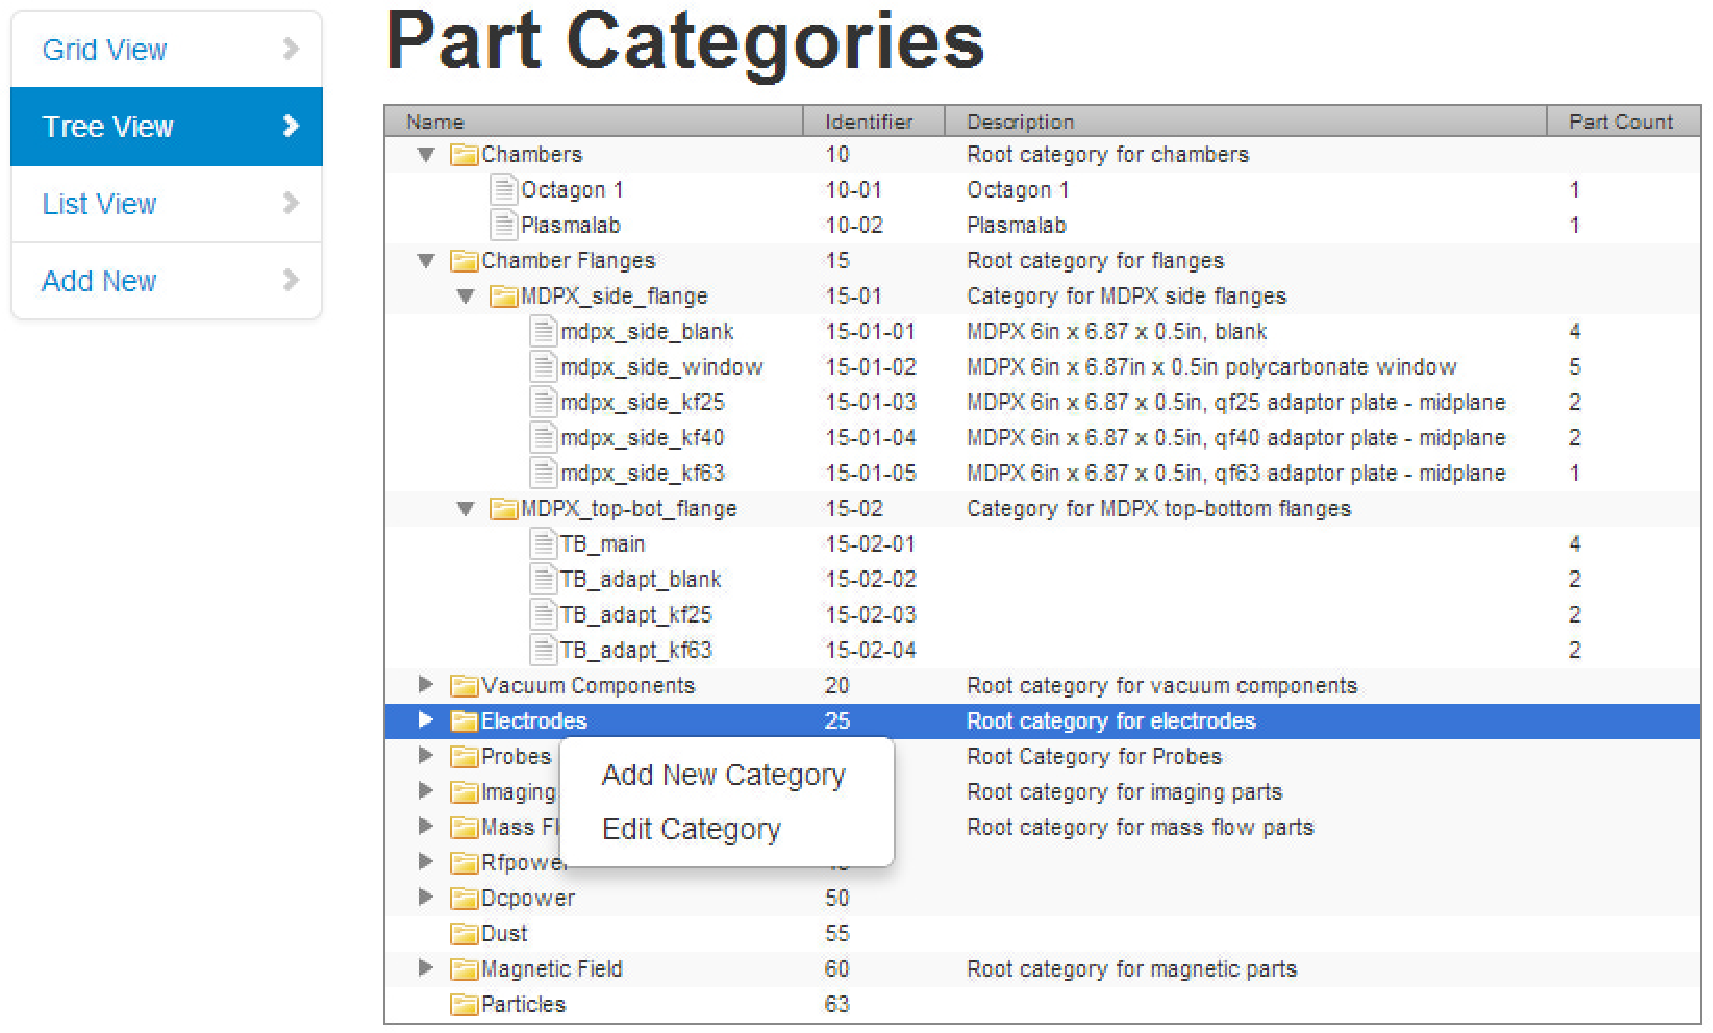
\includegraphics[width=3.5in]{partcat.pdf}
\caption{Tree view of the part categories.\label{fig:partcat}}
\end{figure}

The web interface is implemented via PHP 5.3 with Yii Framework 1.1. The framework provides agnostic database access; therefore, RDBMS from different vendors can be used as the data store. The RDBMS that are supported include MySQL(what we use), PostgreSQL, SQLite, Microsoft SQLServer.

\subsection{Inserting and Modifying Data}

The interface facilitates entering new data into the database as shown in the Figure~\ref{fig:create_exp_setup}.

\begin{figure}[h]
\centering
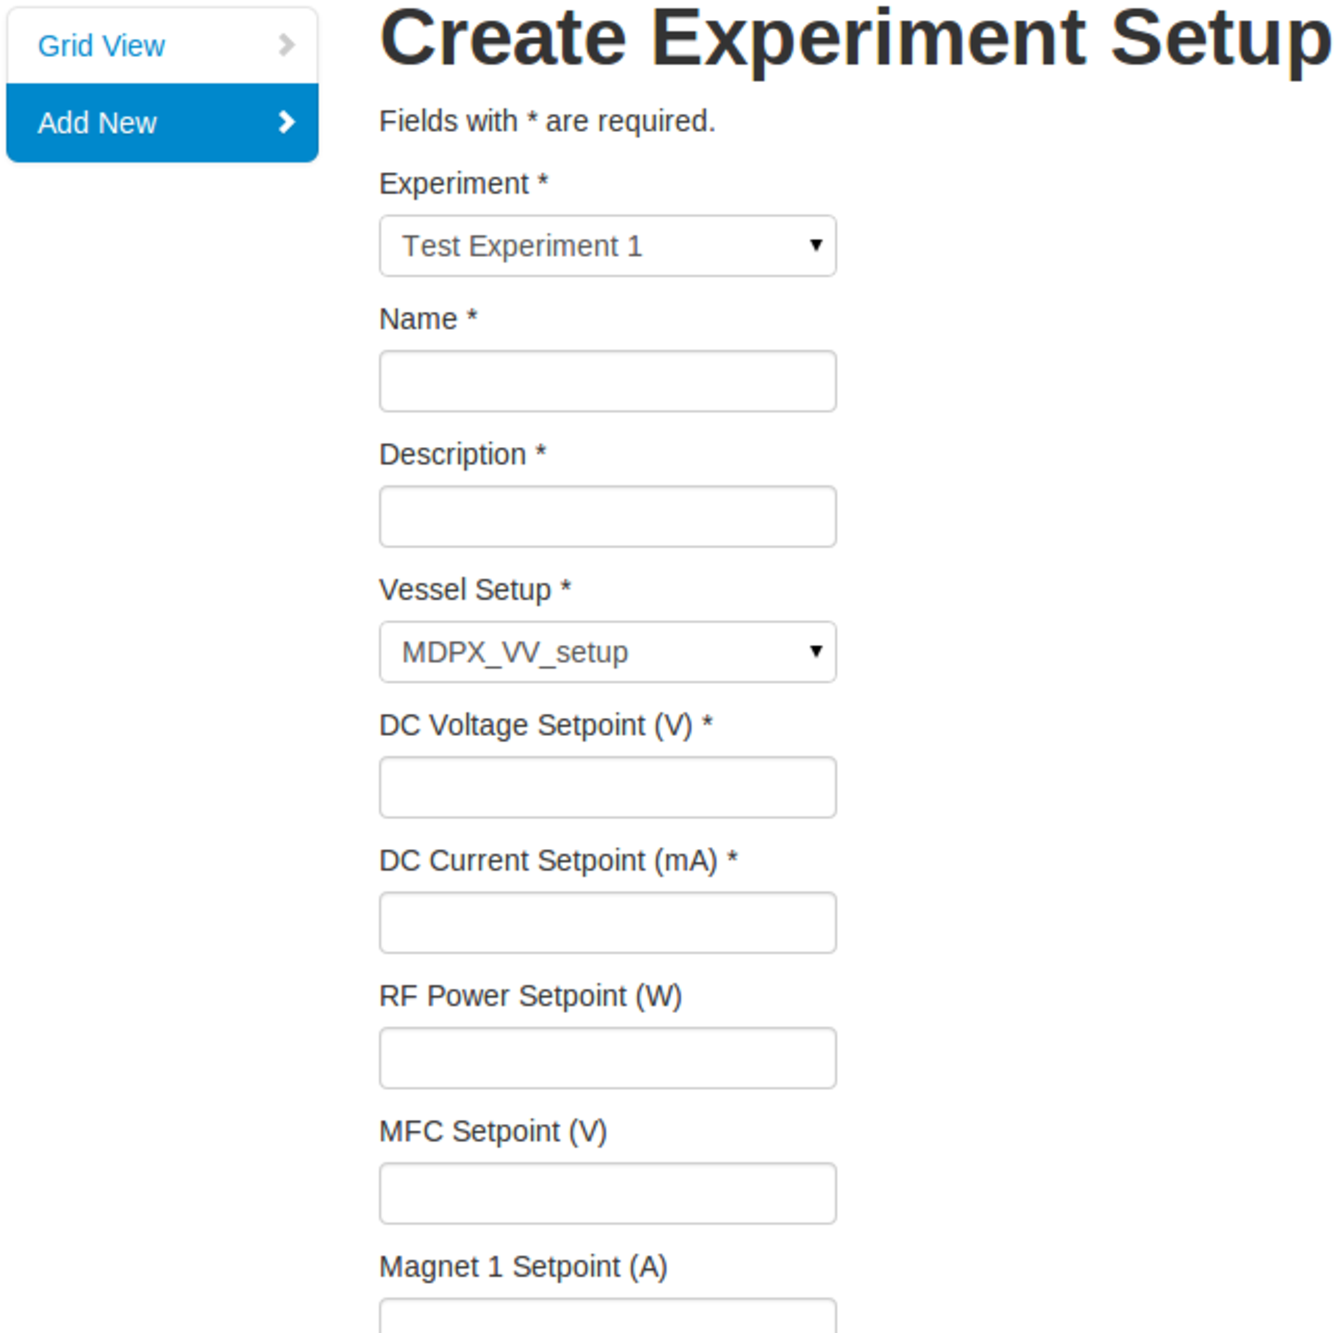
\includegraphics[width=3.5in]{create_experiment_setup.pdf}
\caption{Data entry form and data validation.\label{fig:create_exp_setup}}
\end{figure}

Two ways that the interface make entering and modifying data easier and less error-prone.

The first is that data input form provides selection drop-down menu for data item when possible. The content of these selection menus are usually populated from tables in the database. For example, to insert a new entry into the Experiments table (a experiment group), a researcher and operator user ID is needed. The data entry interface provides a selection menu for these fields so that the user does not have to perform additional step of looking up user IDs. When the data is submitted, the interface inserts the correct user IDs.

The second is that, the interface provides data validation. If a data item does not match a format or validation rule, the data is rejected and will not be saved to the database. The database also enforces data integrity rules. The interface adds a second layer of data integrity and constraint checks.

\subsection{Data Filtering and Searching}

Data filtering is supported in grid views. Figure~\ref{fig:grid_filter} shows the grid view of parts in the system. Users can specify filtering criteria on the columns at the top of the grid view. For string columns, the user can enter the complete or partial search string. For example, to search and researcher with the last name of "Thomas", the user can enter either "Thomas" or just "Thom" as filtering string. For numerical columns, comparison operators (<, >) can be used in filtering criteria.

\begin{figure}[h]
\centering
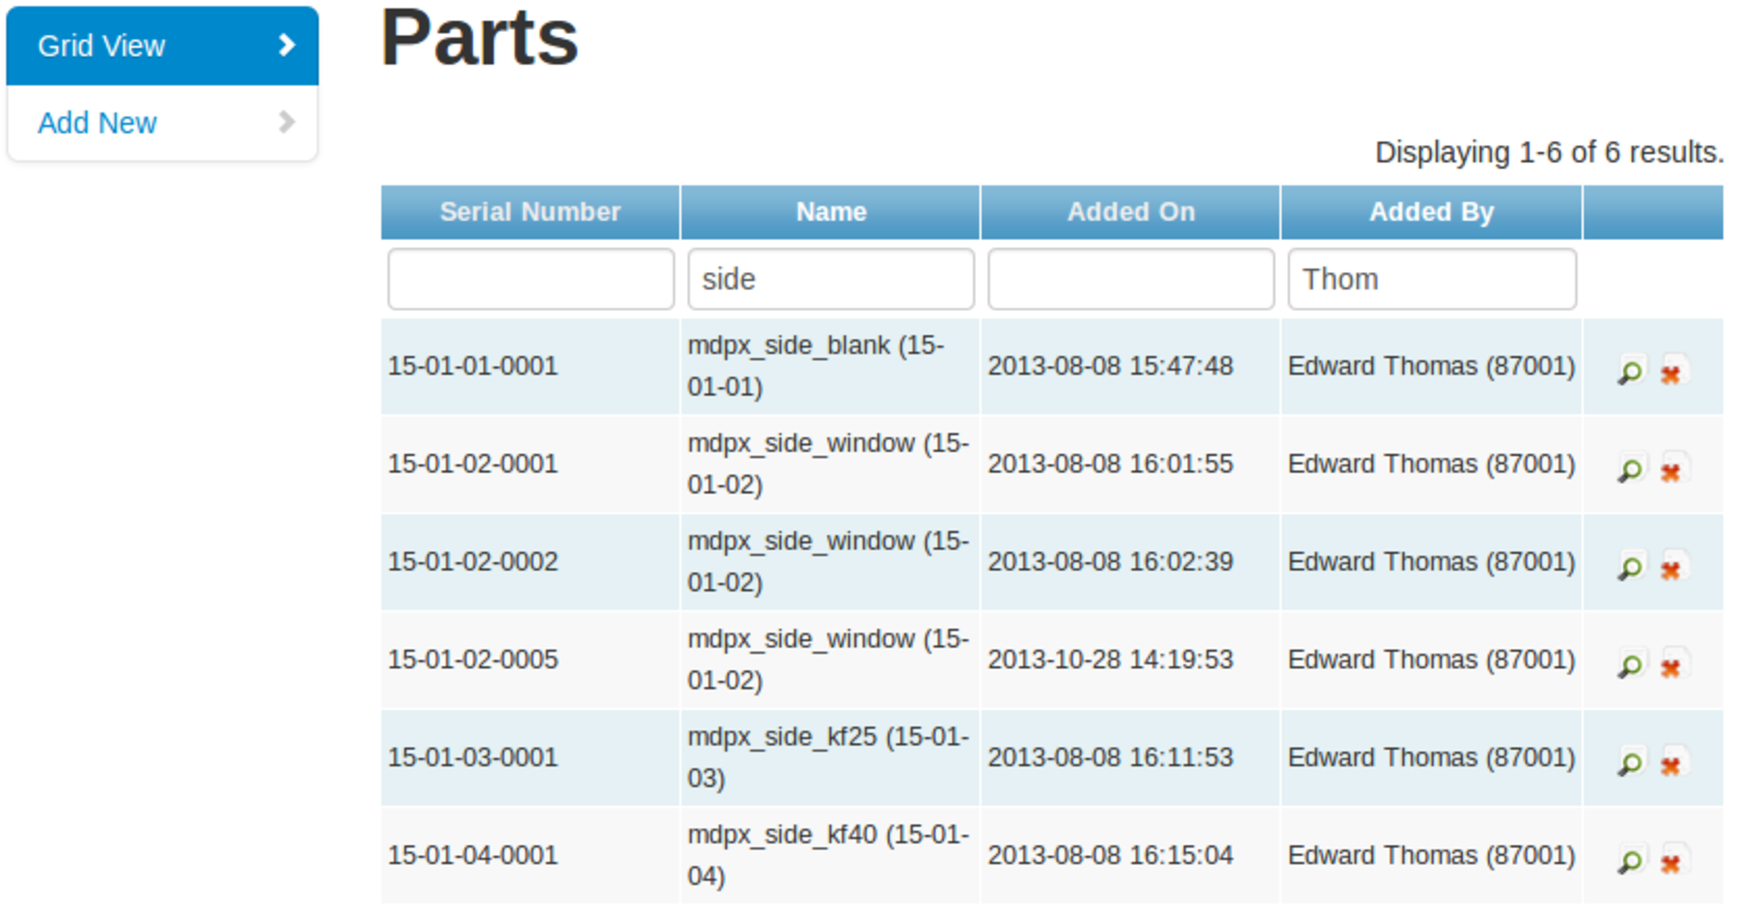
\includegraphics[width=3.5in]{grid_filter.pdf}
\caption{Data Filtering.\label{fig:grid_filter}}
\end{figure}


\onecolumn
\appendix
\section{Database Tables}\label{app_db_schema}

\begin{figure*}[h]
\centering
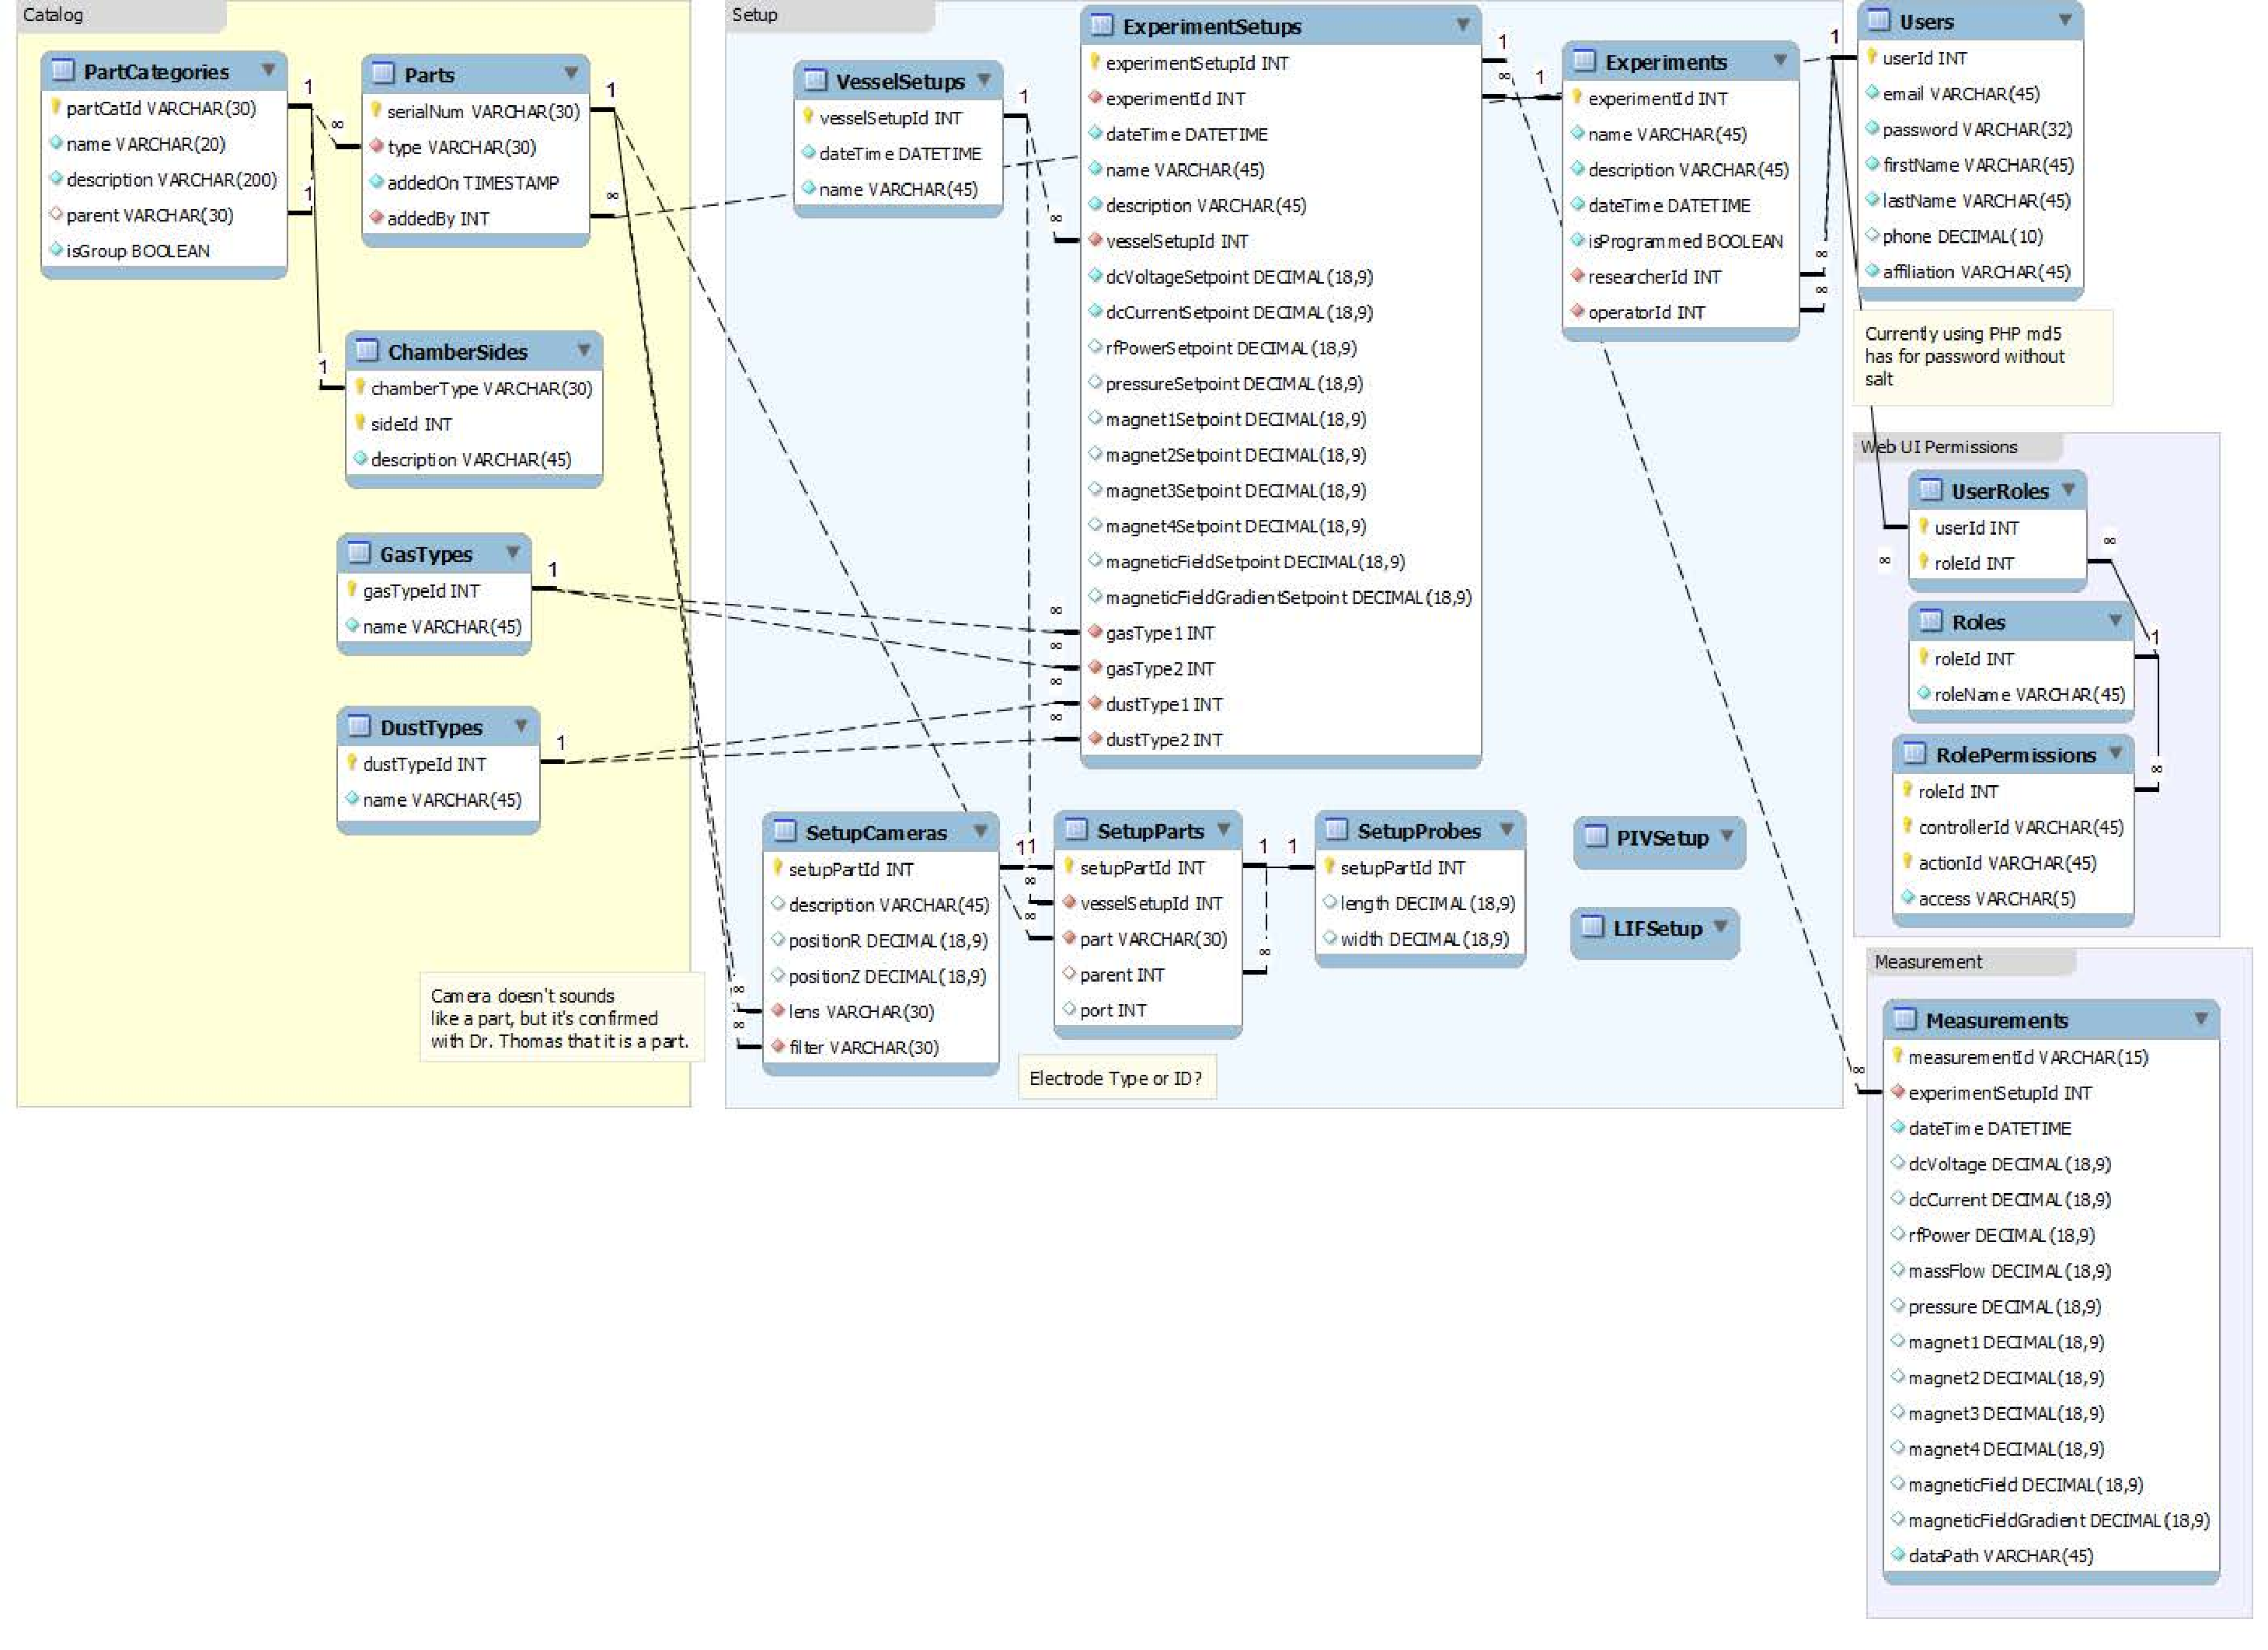
\includegraphics[width=6in]{schema.pdf}
\caption{Database schema.\label{fig:schema}}
\end{figure*}

%\begin{figure}[h!]
%\begin{center}
%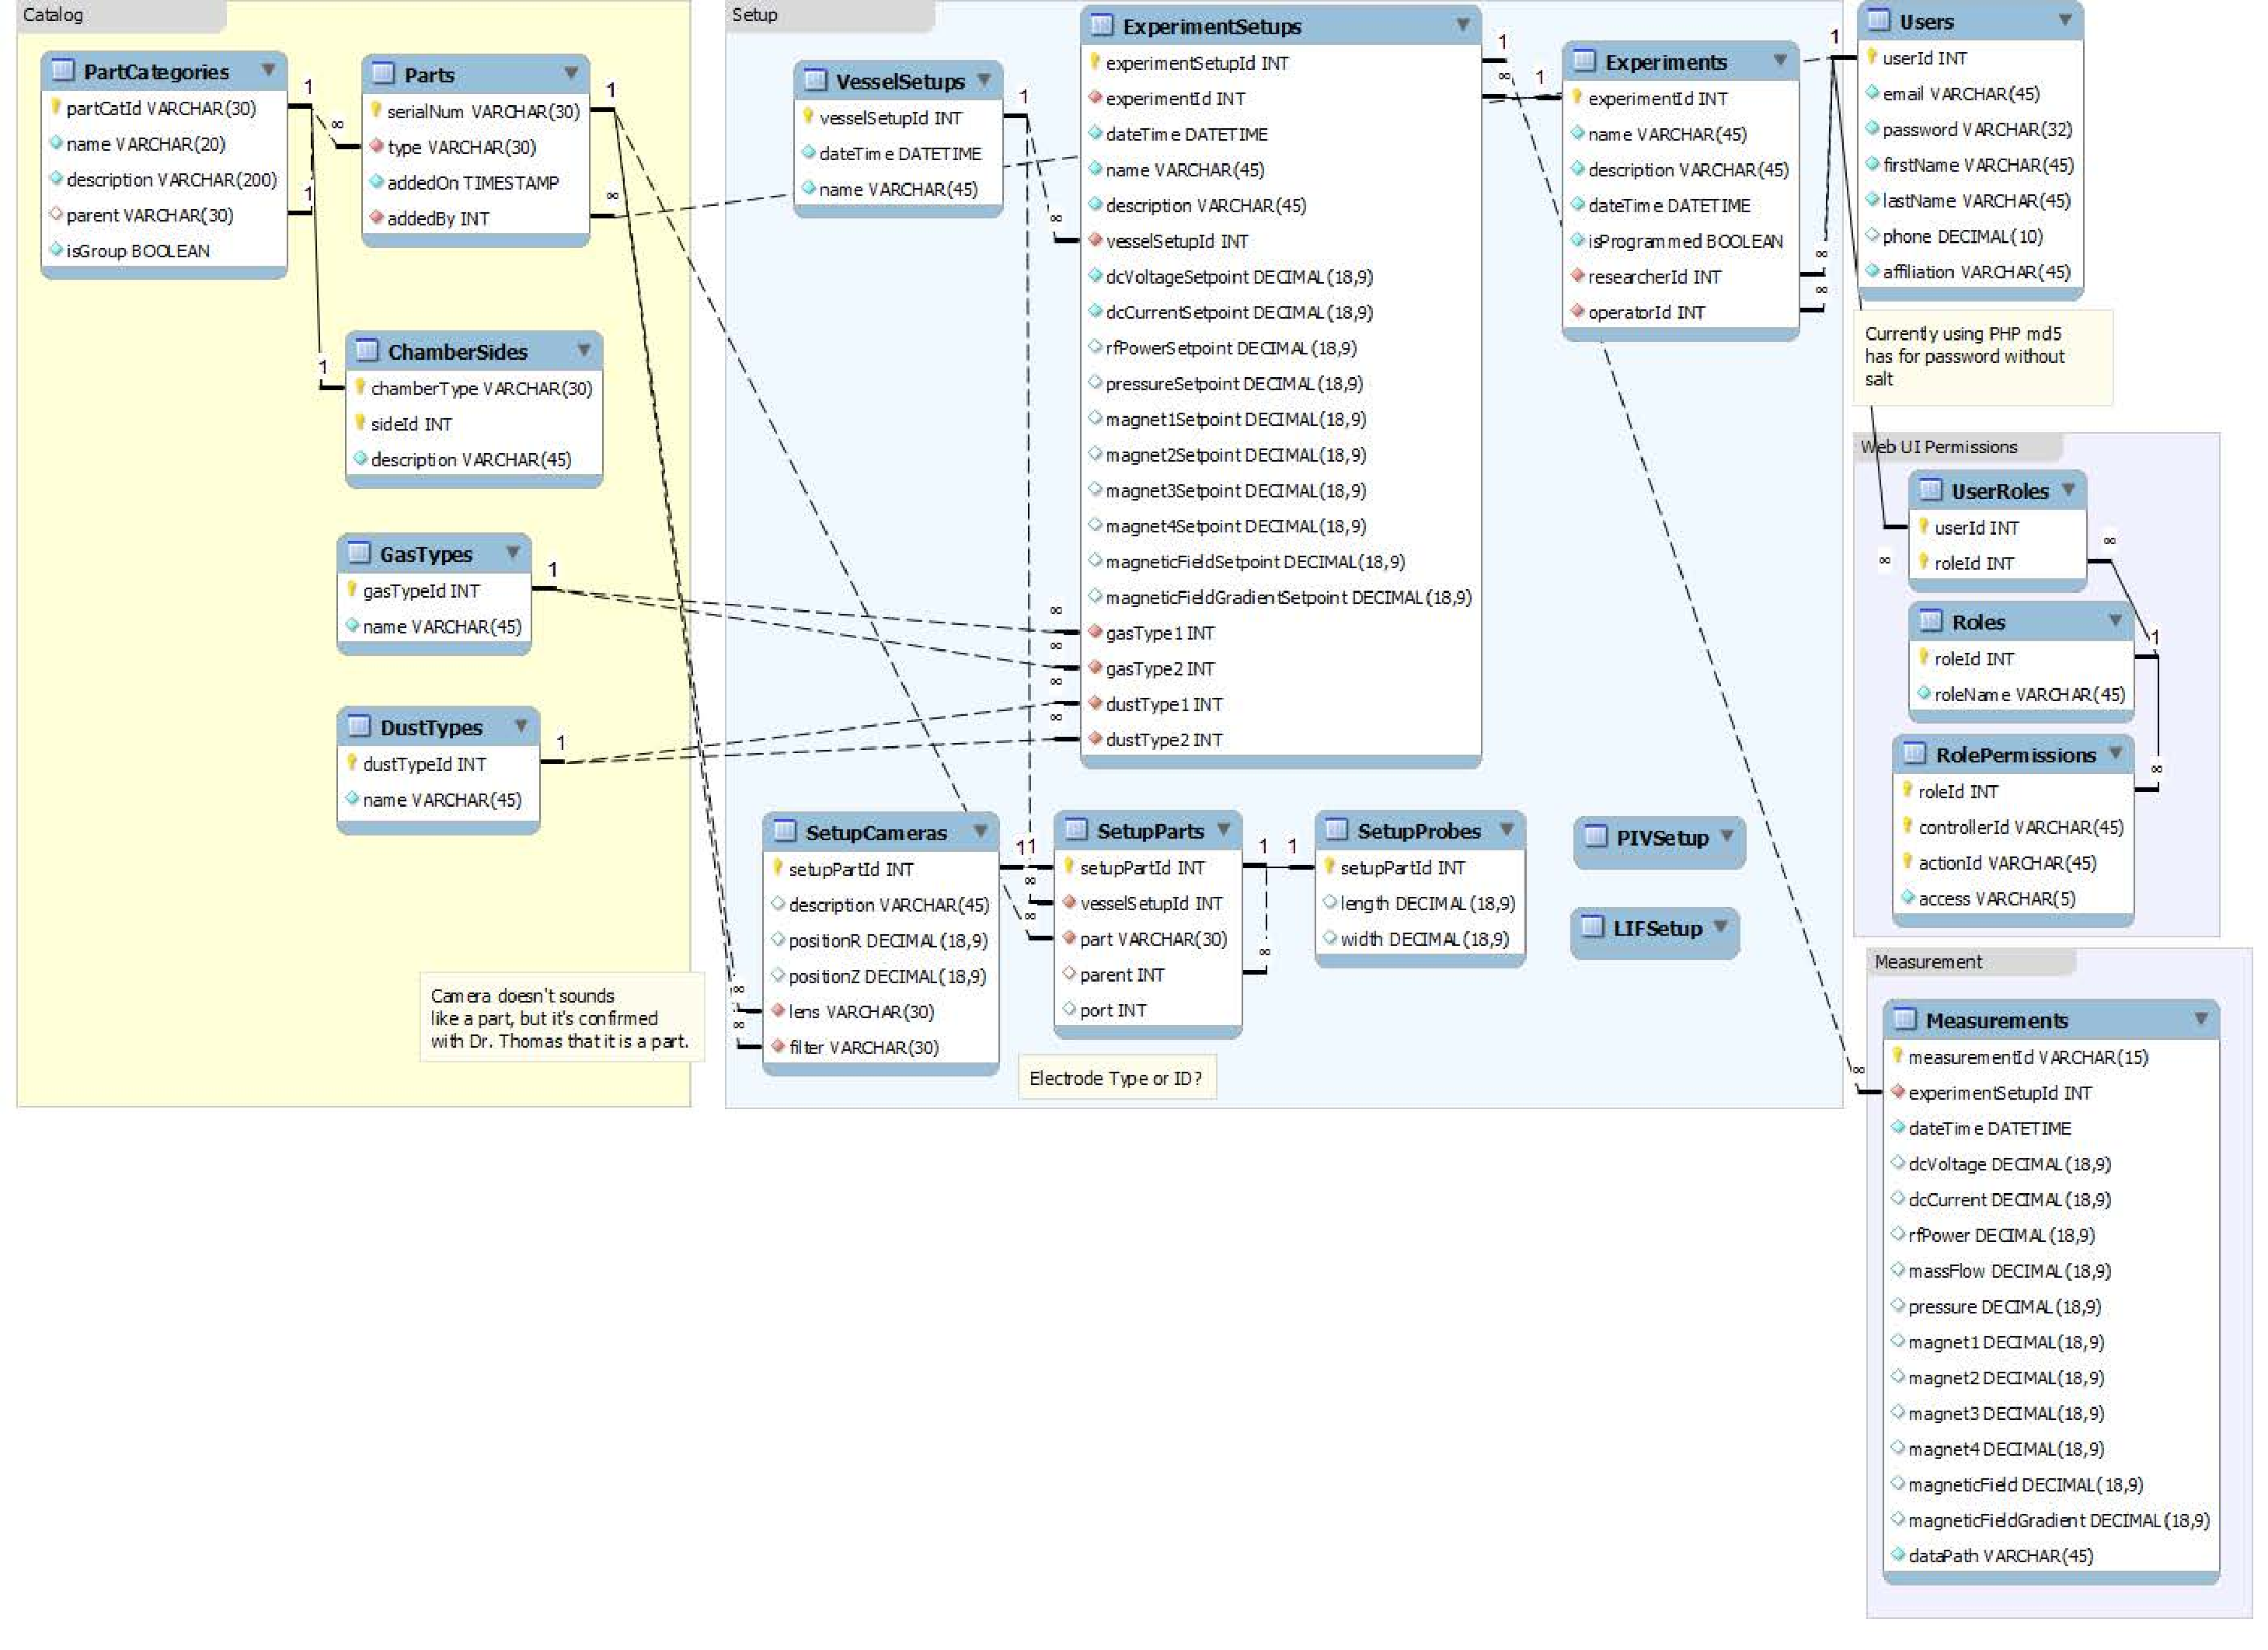
\includegraphics[width=6in]{schema.pdf}
%\caption{Database schema.\label{fig:schema}}
%\end{center}
%\end{figure}

\twocolumn

\section{Database Column Description}

\begin{table}[h!]
\centering
%\caption{PartCategories Table}\label{tb_tables_in_access}
\begin{tabular}{l p{6cm}}
\multicolumn{2}{c}{\bf PartCategories Table} \\ \hline
{\bf Column} & {\bf Description}\\ \hline
partCatId & Identifier of part category.\\ \hline
name & Display name of part category.\\ \hline
description & A textual description of this part category. \\ \hline
parent & Contains Part Category ID of the parent part category node.\\ \hline
isGroup & Denotes if a Part Category is an intermediate node or a leaf node. \\ \hline
\end{tabular}
\end{table}

\begin{table}[h!]
\centering
%\caption{PartCategories Table}\label{tb_tables_in_access}
\begin{tabular}{l p{6cm}}
\multicolumn{2}{c}{\bf Parts Table} \\ \hline
{\bf Column} & {\bf Description}\\ \hline
serialNum & Unique identifier of each part. TWo physical parts of the same type in the catalog will have the same category ID, but different serial number.\\ \hline
type & Part Category ID.\\ \hline
addedOn & The date and time when the part is added to the catalog. \\ \hline
addedBy & The ID of the user who added the part to the catalog.\\ \hline
\end{tabular}
\end{table}

\begin{table}[h!]
\centering
%\caption{PartCategories Table}\label{tb_tables_in_access}
\begin{tabular}{l p{6cm}}
\multicolumn{2}{c}{\bf GasTypes Table} \\ \hline
{\bf Column} & {\bf Description}\\ \hline
gasTypeId & Unique integer identifier.\\ \hline
name & Name of the gas, e.g. Argon.\\ \hline
\end{tabular}
\end{table}

\begin{table}[h!]
\centering
%\caption{PartCategories Table}\label{tb_tables_in_access}
\begin{tabular}{l p{6cm}}
\multicolumn{2}{c}{\bf DustTypes Table} \\ \hline
{\bf Column} & {\bf Description}\\ \hline
gasTypeId & Unique integer identifier.\\ \hline
name & Name of the particle, e.g. Silica 0.5.\\ \hline
\end{tabular}
\end{table}

\begin{table}[h!]
\centering
%\caption{PartCategories Table}\label{tb_tables_in_access}
\begin{tabular}{l p{6cm}}
\multicolumn{2}{c}{\bf VesselSetups Table} \\ \hline
{\bf Column} & {\bf Description}\\ \hline
vesselSetupId & Unique integer database record identifier.\\ \hline
dateTime & Date and time when this setup was created.\\ \hline
name & A descriptive name of this setup.\\ \hline
\end{tabular}
\end{table}

\begin{table}[h!]
\centering
%\caption{PartCategories Table}\label{tb_tables_in_access}
\begin{tabular}{l p{6cm}}
\multicolumn{2}{c}{\bf SetupParts Table} \\ \hline
{\bf Column} & {\bf Description}\\ \hline
setupPartId & Unique integer database record identifier.\\ \hline
vesselSetupId & The ID of the vessel setup to which this part is attached.\\ \hline
part & Serial number of this part.\\ \hline
parent & The ID of the setup part to which this part is attached.\\ \hline
port & The location on the parent part on which this part is attached.\\ \hline
\end{tabular}
\end{table}

\begin{table}[h!]
\centering
%\caption{PartCategories Table}\label{tb_tables_in_access}
\begin{tabular}{l l p{4.6cm}}
\multicolumn{3}{c}{\bf SetupCameras Table} \\ \hline
{\bf Column} & {\bf Unit} & {\bf Description}\\ \hline
setupPartId & & The ID of the setup part of which this record is describing.\\ \hline
description & & Description of the camera.\\ \hline
positionR & Degree & The R position of the camera.\\ \hline
positionZ & Centimeter & The Z position of the camera.\\ \hline
\end{tabular}
\end{table}

\begin{table}[h!]
\centering
%\caption{PartCategories Table}\label{tb_tables_in_access}
\begin{tabular}{l l p{4.6cm}}
\multicolumn{3}{c}{\bf SetupProbes Table} \\ \hline
{\bf Column} & {\bf Unit} & {\bf Description}\\ \hline
setupPartId & & The ID of the setup part of which this record is describing.\\ \hline
length & Centimeter & The length of the probe.\\ \hline
width & Centimeter & The width of the probe.\\ \hline
\end{tabular}
\end{table}

\begin{table}[h!]
\centering
%\caption{ExperimentSetups Table}\label{tb_tables_in_access}
\begin{tabular}{l l p{2.5cm}}
\multicolumn{3}{c}{\bf ExperimentSetups Table} \\ \hline
{\bf Column} & {\bf Unit} & {\bf Description}\\ \hline
experimentSetupId & & Unique integer database record identifier.\\ \hline
experimentId & & ID of an record in Experiments table.\\ \hline
dateTime & & Date and time on which this setup was created.\\ \hline
name & & Descriptive name.\\ \hline
description & & Description.\\ \hline
vesselSetupId & & Database ID of the vessel setup of this experiment.\\ \hline
dcVoltageSetpoint & Volt & \\ \hline
dcCurrentSetpoint & Milliamp & \\ \hline
rfPowerSetpoint & Watt & \\ \hline
pressureSetpoint & Volt & \\ \hline
magnet1Setpoint & Amp & \\ \hline
magnet2Setpoint & Amp & \\ \hline
magnet3Setpoint & Amp & \\ \hline
magnet4Setpoint & Amp & \\ \hline
magneticFieldSetpoint & Tesla & \\ \hline
magneticFieldGradientSetpoint & Tesla/Meter & \\ \hline
gasType1 && \\ \hline
gasType2 && \\ \hline
dustType1 && \\ \hline
dustType2 && \\ \hline
\end{tabular}
\end{table}

\begin{table}[h!]
\centering
%\caption{Experiments Table}\label{tb_tables_in_access}
\begin{tabular}{l p{6cm}}
\multicolumn{2}{c}{\bf Experiments Table} \\ \hline
{\bf Column} & {\bf Description}\\ \hline
experimentId & Unique integer database record identifier.\\ \hline
name & Descriptive name of the experiment group.\\ \hline
description & Description of the experiment group.\\ \hline
dateTime & The date and time on which this group was created.\\ \hline
isProgrammed & A boolean flag that signifies if this group of experiment is conducted by a program that iterates through a range of values for a set of paramenters.\\ \hline
description & Description of the experiment group.\\ \hline
researcherId & Foreign key to Users.userId. This means each record in this table has a researcher.\\ \hline
operatorId & Foreign key to Users.userId. This means each record in this table has an operator.\\ \hline
\end{tabular}
\end{table}

\begin{table}[h!]
\centering
%\caption{Measurements Table}\label{tb_tables_in_access}
\begin{tabular}{l l p{3cm}}
\multicolumn{3}{c}{\bf Measurements Table} \\ \hline
{\bf Column} & {\bf Unit} & {\bf Description}\\ \hline
measurementId & & Primary key of this table.\\ \hline
experimentSetupId & & Foreign key to ExperimentSetups.experimentSetupId. This relationship means every measurement is linked with one experiment setup, and every experiment setup has multiple measurements.\\ \hline
dateTime & & Date and time when a record was recorded.\\ \hline
dcVoltage & Volt & Monitored average DC voltage of ...?\\ \hline
dcCurrent & Milliamp & Monitored average DC current of ...?\\ \hline
rfPower & Watt & \\ \hline
massFlow & Volt & \\ \hline
pressure & ? & \\ \hline
magnet1 & Ampere & \\ \hline
magnet2 & Ampere & \\ \hline
magnet3 & Ampere & \\ \hline
magnet4 & Ampere & \\ \hline
magneticField & Tesla & \\ \hline
magneticFieldGradient & Tesla/Meter & \\ \hline
dataPath & & Where the corresponding data is stored.\\ \hline
\end{tabular}
\end{table}

\begin{table}[h!]
\centering
%\caption{PartCategories Table}\label{tb_tables_in_access}
\begin{tabular}{l p{6cm}}
\multicolumn{2}{c}{\bf Users Table} \\ \hline
{\bf Column} & {\bf Description}\\ \hline
userId & Primary key for this table.\\ \hline
email & Email address of this user.\\ \hline
password & Password of the user hashed using md5 without salt.\\ \hline
firstName & First name of the user.\\ \hline
lastName & Last name of the user.\\ \hline
phone & Contact telephone number of the user.\\ \hline
affiliation & Associated organization of the user.\\ \hline
\end{tabular}
\end{table}

\begin{table}[h!]
\centering
%\caption{PartCategories Table}\label{tb_tables_in_access}
\begin{tabular}{l p{6cm}}
\multicolumn{2}{c}{\bf Roles Table} \\ \hline
{\bf Column} & {\bf Description}\\ \hline
roleId & Primary key for this table.\\ \hline
roleName & Name of this role, e.g. Admin.\\ \hline
\end{tabular}
\end{table}

\begin{table}[h!]
\centering
%\caption{PartCategories Table}\label{tb_tables_in_access}
\begin{tabular}{l p{6cm}}
\multicolumn{2}{c}{\bf RolePermissions Table} \\ \hline
{\bf Column} & {\bf Description}\\ \hline
roleId & Foreign key to Roles.roleId. This means for reach \\ \hline
controllerId & Controller identifier of the web interface.\\ \hline
actionId & Action identifier of the web interface.\\ \hline
access & Have value of either ALLOW or DENY. This column specifies whether an operation identified by pair {controllerId, actionId} can be performed by a role.\\ \hline
\end{tabular}
\end{table}

\clearpage

\small {\section*{Acknowledgments}

This research has been funded in part by the National Science
Foundation grants CNS-0831502 (CT) and CNS-0855251 (CRI).}

\small{
\bibliographystyle{abbrv}
\bibliography{ref}
}
\end{document}
